\documentclass[../capitulos/cap1.tex]{subfiles}

\tikzset{every picture/.style={line width=0.75pt}} %set default line width to 0.75pt        

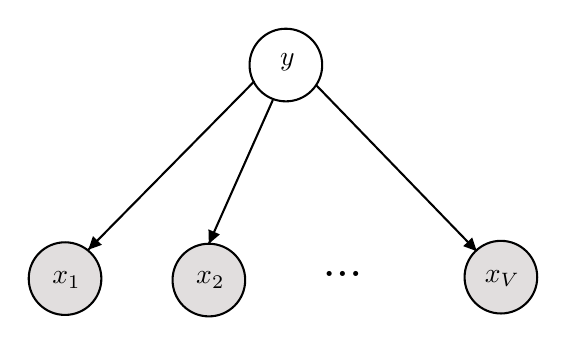
\begin{tikzpicture}[x=0.75pt,y=0.75pt,yscale=-0.7,xscale= 0.7]
%uncomment if require: \path (0,300); %set diagram left start at 0, and has height of 300

\draw    (338, 37) circle [x radius= 25, y radius= 25]  ;
\draw  [fill={rgb, 255:red, 225; green, 222; blue, 222 }  ,fill opacity=1 ]  (285, 185) circle [x radius= 25, y radius= 25]  ;
\draw  [fill={rgb, 255:red, 225; green, 222; blue, 222 }  ,fill opacity=1 ]  (186, 184) circle [x radius= 25, y radius= 25]  ;
\draw  [fill={rgb, 255:red, 225; green, 222; blue, 222 }  ,fill opacity=1 ]  (486, 183) circle [x radius= 25, y radius= 25]  ;
\draw    (316.38,48.11) -- (202.02,164.11) ;
\draw [shift={(202.02,164.11)}, rotate = 314.59000000000003] [fill={rgb, 255:red, 0; green, 0; blue, 0 }  ] [draw opacity=0] (8.93,-4.29) -- (0,0) -- (8.93,4.29) -- (8.93,-4.29)    ;

\draw    (329.02,61.11) -- (285,160) ;
\draw [shift={(285,160)}, rotate = 293.99] [fill={rgb, 255:red, 0; green, 0; blue, 0 }  ] [draw opacity=0] (8.93,-4.29) -- (0,0) -- (8.93,4.29) -- (8.93,-4.29)    ;

\draw    (359,51) -- (469.38,165.11) ;
\draw [shift={(469.38,165.11)}, rotate = 225.95] [fill={rgb, 255:red, 0; green, 0; blue, 0 }  ] [draw opacity=0] (8.93,-4.29) -- (0,0) -- (8.93,4.29) -- (8.93,-4.29)    ;


\draw (377,181) node [scale=1.7280000000000002] [align=left] {...};
\draw (339,35) node   {$y$};
\draw (187,185) node   {$x_{1}$};
\draw (286,185) node   {$x_{2}$};
\draw (487,184) node   {$x_{V}$};


\end{tikzpicture}